\chapter{Specialising and optimising xDSL pattern rewriting}
\label{chap:specialising-optimising-pattern-rewriting}

%% Introduction and goals (make faster and only constrained by language runtime)
% Hook
In \autoref{chap:measuring-compiler-performance}, we constructed a set of experiments to empirically compare the current performance of the xDSL and MLIR compiler frameworks.
% Argument
The goal of these experiments is to use xDSL and MLIR as proxies to characterise the performance of static and dynamic languages for the implementation of user-extensible compiler frameworks.
However, these experiments do not exactly capture this goal. We argue this is because they are measuring both the implementation details of the framework in addition to the runtime of the language, with the former obscuring our goal of measuring the latter.
% The results of these experiments showed that two factors contributed to the slow-down between the MLIR and xDSL frameworks: overhead incurred by the Python language runtime, and design choices made when implementing xDSL.
% In order to use the xDSL and MLIR frameworks to understand the performance of static and dynamic languages for the implementation of user-extensible compiler frameworks, our measurements must be as independent of implementation details as possible.
In this chapter, we mitigate this by specialising the xDSL framework to implement only a single workload. This elides aspects of the implementation which provide expressivity at the cost of performance, and is representative of the best-case performance of Python for this workload.
% Link
The benefits of this specialisation are twofold. Firstly it reveals inefficiencies in xDSL which can be optimised to improve the general performance of the framework. Secondly, it provides a true performance baseline for dynamic languages irrespective of implementation details which can be used to quantify the impact of dynamism in \autoref{chap:dynamism-pattern-rewriting}.



\section{Micro-benchmarks}
\label{sec:specialising-ubenchmarks}

%% Link back to micro-benchmarks and summarise section
% Hook
An important component of our experimental suite is micro-benchmarks, measuring the performance of operations fundamental to xDSL and MLIR.
% Argument
The small size of these micro-benchmarked fundamental operations makes them tractable first targets for manual specialisation and optimisation, with the performance impact of this process easily characterised by repeating the micro-benchmark.
% Link
In this section, we examine the specialisation process for these micro-benchmarks in detail. % TODO: Add more stuff here!!


\subsection{Operation instantiation}
\label{sec:specialising-ubenchmarks-instantiation}

%% Re-introduce microbenchmark
% Hook
% Argument
% Link

\begin{figure}[H]
    \begin{subfigure}[b]{0.4\textwidth}
       \centering
        \begin{minted}[fontsize=\footnotesize,escapeinside=$$]{text}
            ConstantOp(
                IntegerAttr(
                    100,
                    i32
                )
            )
        \end{minted}
        \footnotesize\vspace{3em}
        \caption{Instantiation with constructors.}
        \label{listing:ubenchmark-xdsl-constant-constructor}
    \end{subfigure}
    \hfill
    \begin{subfigure}[b]{0.6\textwidth}
        \centering
        \begin{minted}[breakanywhere,fontsize=\footnotesize,escapeinside=$$]{text}
            int_attr = IntAttr.__new__(IntAttr)
            object.__setattr__(int_attr, "data", 100)
            integer_attr = IntegerAttr.__new__(IntegerAttr)
            object.__setattr__(integer_attr, "parameters", (int_attr, i32))
            constant_op = ConstantOp.__new__(ConstantOp)
            constant_op._operands = tuple()
            constant_op.results = (OpResult(i32, constant_op, 0),)
            constant_op.properties = {"value": integer_attr}
            constant_op.attributes = {}
            constant_op._successors = []
            constant_op.regions = tuple()
        \end{minted}
        \caption{Instantiation by direct manipulation of xDSL's data structures.}
        \label{listing:ubenchmark-xdsl-constant-direct}
    \end{subfigure}
    \captionsetup{name=Listing}
    \caption{Approaches to instantiating an arithmetic constant.}
    \label{listing:ubenchmark-xdsl-constant}
\end{figure}

%% Describe specialisation/optimisation
% Hook
% Argument
% Link

\begin{figure}[H]
    \centering
    \begin{subfigure}[b]{\textwidth}
        \centering
        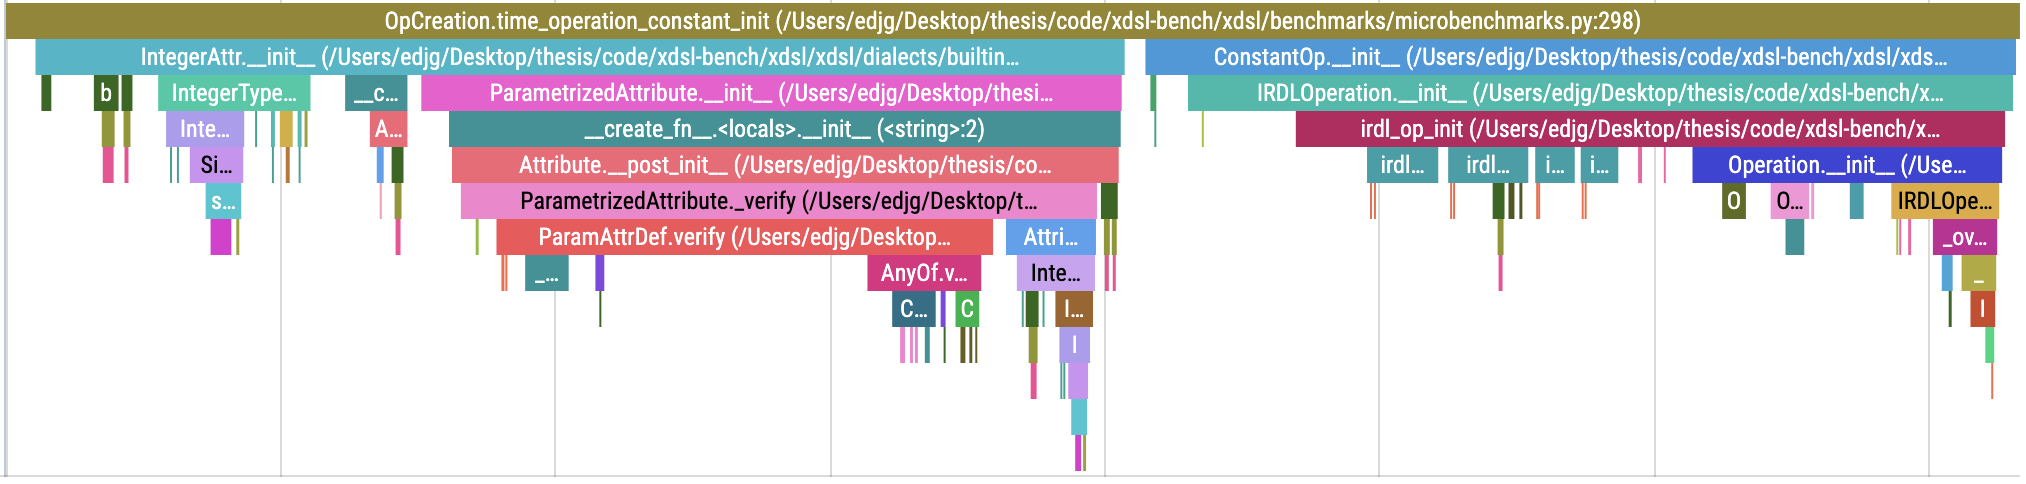
\includegraphics[width=\textwidth]{images/specialising_optimising_xdsl_rewriting/original_constant_create.png}
        \captionsetup{width=0.8\textwidth}
        \caption{.}
        \label{fig:ubenchmark-hastrait-xdsl-viztracer}
    \end{subfigure}
    \begin{subfigure}[b]{\textwidth}
        \centering
        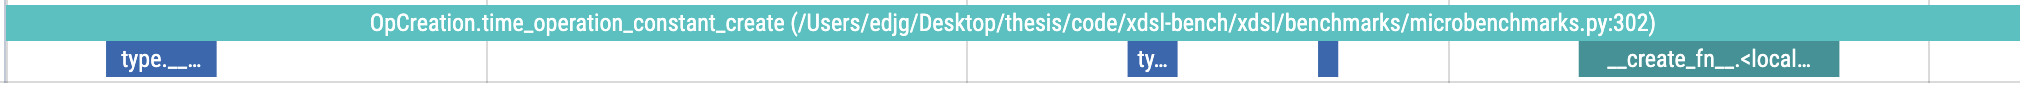
\includegraphics[width=\textwidth]{images/specialising_optimising_xdsl_rewriting/optimised_constant_create.png}
        \captionsetup{width=0.8\textwidth}
        \caption{.}
        \label{fig:ubenchmark-gettrait-xdsl-viztracer}
    \end{subfigure}
    \caption{.}
    \label{fig:ubenchmark-hasgettrait-xdsl-viztracer}
\end{figure}

\begin{table}[H]
  \caption{.}
  \label{tab:ubenchmark-instantiation-optimised}
  \centering
  \begin{tabular}{ccc}
    \toprule
    \textbf{MLIR [ns]} & \textbf{xDSL [ns]} & \textbf{Optimised xDSL [ns]} \\
    \midrule
    $3.89 \pm 0.01$ & $504 \pm 76$ & $63.6 \pm 40$\\
    \bottomrule
  \end{tabular}
\end{table}

%% Specialised performance and lessons learnt
% Hook
% Argument
% Link
From this example, we can see that xDSL's design goal of a simple, expressive API is antagonistic with the performance of its implementation. By specialising the implementation to the workload, directly invoking only the required instructions, we can achieve significant performance improvements. We argue that this specialisation approaches the upper bound of performance for this workload as a result of the constraints of the language runtime.










\subsection{Operation trait checks}
\label{ssec:specialising-ubenchmarks-trait}

%% Re-introduce microbenchmark
% Hook
The second micro-benchmark discussed in \autoref{sec:ubenchmark} was checking traits on operations, and was measured to perform $\times$ worse in xDSL than MLIR -- a slow-down significantly greater than other micro-benchmarks.
% Argument
This suggests that the implementation of the \mintinline{python}{has_trait} method (Listing \ref{listing:ubenchmark-trait-checks-xdsl}) has room for optimisation before it is bound only by the language runtime.
In this method,
% Link

\begin{figure}[H]
    \begin{subfigure}[b]{0.45\textwidth}
       \centering
        \begin{minted}[fontsize=\footnotesize,escapeinside=$$]{text}
            @classmethod
            def has_trait(
                cls,
                trait: type[OpTrait] | OpTrait,
                *,
                value_if_unregistered: bool = True,
            ) -> bool:
                from xdsl.dialects.builtin import UnregisteredOp $\circledbase{pairedOneLightBlue}{1}$

                if issubclass(cls, UnregisteredOp):
                    return value_if_unregistered

                return cls.get_trait(trait) is not None $\circledbase{pairedTwoDarkBlue}{2}$
        \end{minted}
        \footnotesize\vspace{1.5em}
        \caption{Outer \mintinline{python}{has_trait} method.}
        \label{listing:ubenchmark-trait-checks-xdsl-has}
    \end{subfigure}
    \hfill
    \begin{subfigure}[b]{0.45\textwidth}
        \centering
        \begin{minted}[breakanywhere,fontsize=\footnotesize,escapeinside=$$]{text}
            @classmethod
            def get_trait(
                cls,
                trait: type[OpTraitInvT] | OpTraitInvT
            ) -> OpTraitInvT | None:
                if isinstance(trait, type): $\circledbase{pairedThreeLightGreen}{3}$
                    for t in cls.traits:
                        if isinstance(t, cast( $\circledbase{pairedFourDarkGreen}{4}$
                            type[OpTraitInvT], trait
                        )):
                            return t
                else:
                    for t in cls.traits:
                        if t == trait:
                            return cast(OpTraitInvT, t)
                return None
        \end{minted}
        \caption{Inner \mintinline{python}{get_trait} method.}
        \label{listing:ubenchmark-trait-checks-xdsl-get}
    \end{subfigure}
    \vspace{1em}
    \captionsetup{name=Listing}
    \caption{xDSL methods implementing trait check functionality.}
    \label{listing:ubenchmark-trait-checks-xdsl}
\end{figure}


%% Describe specialisation/optimisation
% Hook
% Argument
% Link

\begin{code}
    \centering
    \begin{minted}[fontsize=\footnotesize]{python}
        has_trait = False
        for t in OP.traits._traits:
            if isinstance(t, TRAIT):
                has_trait = True
                break
    \end{minted}
    \footnotesize\vspace{5.5em}
    \captionsetup{name=Listing}
    \caption{xDSL's modified \mintinline{python}{has_trait} method.}
    \label{listing:ubenchmark-trait-checks-xdsl-optimised}
\end{code}

%% Specialised performance and lessons learnt
% Hook
% Argument
% Link

\begin{figure}[H]
    \centering
    \begin{subfigure}[b]{\textwidth}
        \centering
        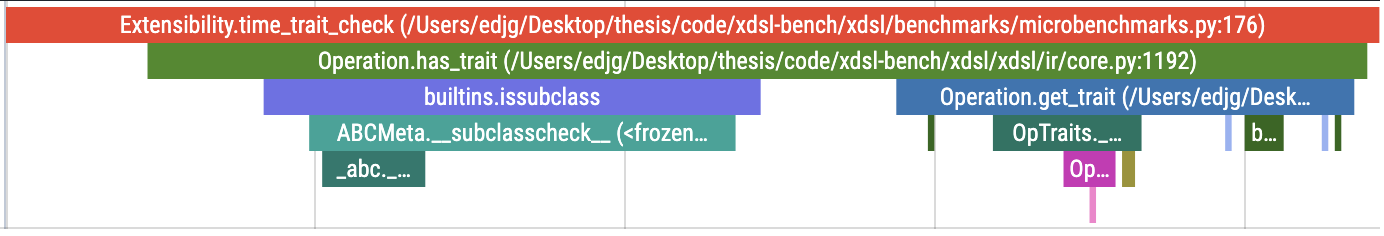
\includegraphics[width=\textwidth]{images/specialising_optimising_xdsl_rewriting/original_hastrait.png}
        \captionsetup{width=0.8\textwidth}
        \caption{\mintinline{python}{issubclass} and \mintinline{python}{isinstance} checks, type \mintinline{python}{cast}ing, and constructing iterators constitutes over three quarters of xDSL's \mintinline{python}{has_trait}s runtime.}
        \label{fig:ubenchmark-hastrait-original-viztracer}
    \end{subfigure}
    \begin{subfigure}[b]{\textwidth}
        \centering
        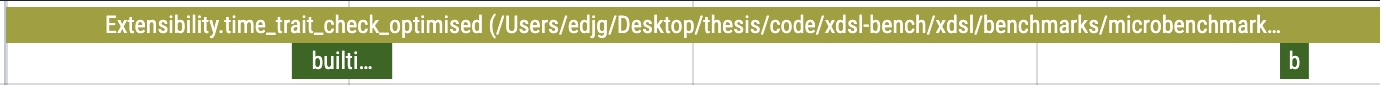
\includegraphics[width=\textwidth]{images/specialising_optimising_xdsl_rewriting/optimised_hastrait.png}
        \captionsetup{width=0.8\textwidth}
        \caption{Specialisation to narrow the interface and optimisation to avoid extraneous work on hot paths can significantly accelerate \mintinline{python}{has_trait}.}
        \label{fig:ubenchmark-hastrait-optimised-viztracer}
    \end{subfigure}
    \caption{\texttt{viztracer} traces of xDSL's \mintinline{python}{has_trait} method.}
    \label{fig:ubenchmark-hastrait-viztracer}
\end{figure}


\begin{table}[H]
  \caption{Trait checks in xDSL are approximately $130\times$ slower than in MLIR in the asymptotic case, but can be accelerated to $16\times$ slower with only algorithmic changes.} %, repeated ten times over $32768$ operations. Methodology is discussed in detail in Appendix \ref{} to facilitate replicability.}
  \label{tab:ubenchmark-trait-checks-optimised}
  \centering
  \begin{tabular}{ccc}
    \toprule
    \textbf{MLIR [ns]} & \textbf{xDSL [ns]} & \textbf{Optimised xDSL [ns]} \\
    \midrule
    $3.89 \pm 0.01$ & $504 \pm 76$ & $63.6 \pm 40$\\
    \bottomrule
  \end{tabular}
\end{table}




\section{Pattern rewriting}
\label{sec:specialising-pattern-rewriting}


\subsection{Constant folding workload}
\label{sec:specialising-pattern-rewriting-workload}

%% Summarise the workload and how it is special (xDSL and MLIR!)
% Link
% Argument
% Link

%% Listing showing the two guys


\subsection{Specialisation}
\label{sec:specialising-pattern-rewriting-specialisation}

%% What does specialisation mean in this context (inlining/eliding/...)
% Link
% Argument
% Link

%% Figure comparing traces

\begin{figure}[H]
    \centering
    \begin{subfigure}[b]{\textwidth}
        \centering
        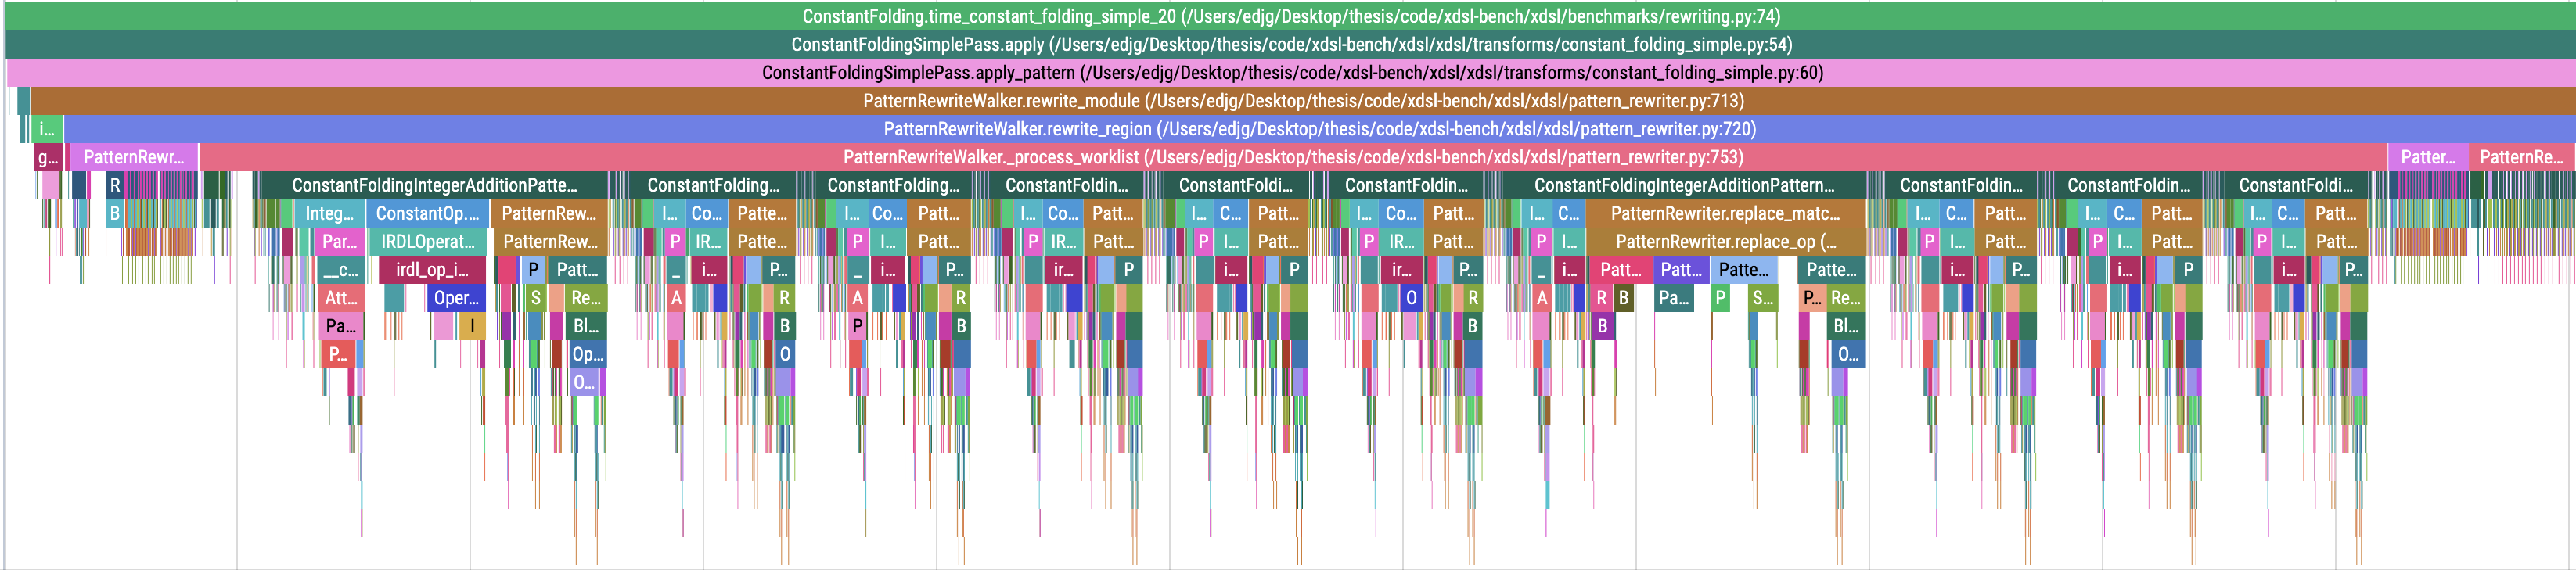
\includegraphics[width=\textwidth]{images/specialising_optimising_xdsl_rewriting/custom_constant_fold.png}
        \captionsetup{width=0.8\textwidth}
        \caption{.}
        \label{fig:constant-fold-original-viztracer}
    \end{subfigure}
    \begin{subfigure}[b]{\textwidth}
        \centering
        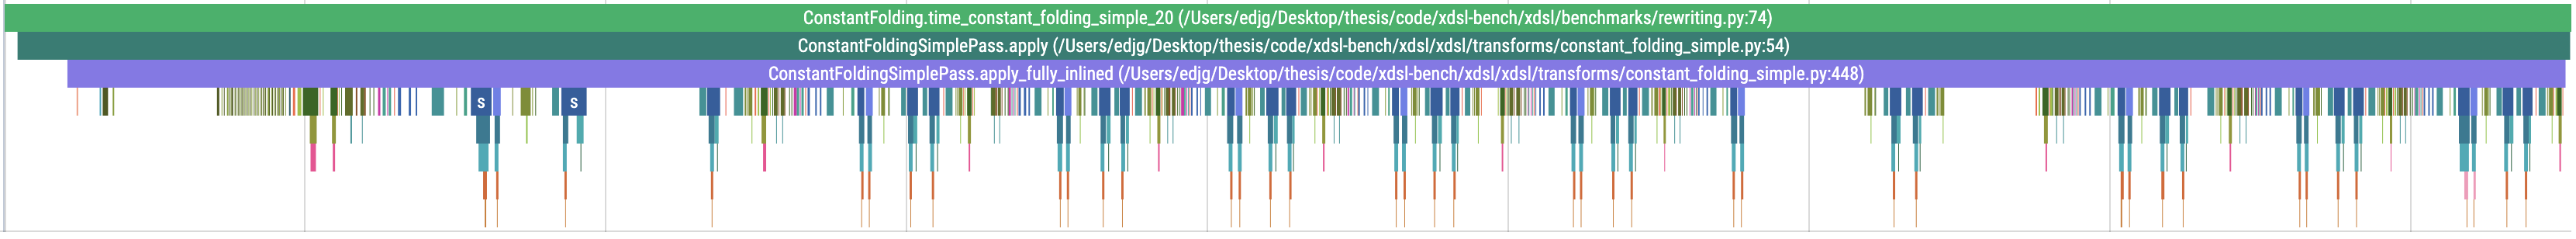
\includegraphics[width=\textwidth]{images/specialising_optimising_xdsl_rewriting/optimised_constant_fold.png}
        \captionsetup{width=0.8\textwidth}
        \caption{.}
        \label{fig:constant-fold-optimised-viztracer}
    \end{subfigure}
    \caption{\texttt{viztracer} traces of.}
    \label{fig:constant-fold-viztracer}
\end{figure}

%% Either perf table here or later in summary?

%% Hopes of automation?
% Link
% Argument
% Link

\subsection{Optimisations}
\label{sec:specialising-pattern-rewriting-optimisations}

%% Introduction + scope of stuff
% Hook
% Argument
% xDSL is very big -- cannot optimise everything! But can show optimisations from specialisation are applicable and make change with time.
% Link


%% Removing overhead in functions
% Link
% Argument
% Link


%% Removing implicit builders
% Link
% Argument
% Link


%% Optional stretch goal to be filled in later...?
%% `__slots__` (stretch dataclasses stuff -> custom dataclass like thing without most of the overhead as a helper, replaces frozen dataclasses (what functionality is used here: https://github.com/python/cpython/blob/main/Lib/dataclasses.py and what can we rip out???))



\subsection{Performance improvement}
\label{sec:specialising-pattern-rewriting-performance}

%% How much did we get out of this?
% Link
% Argument
% Link

%% Figure or table comparing performance
\begin{table}[H]
  \caption{.}
  \label{tab:constant-folding-optimised}
  \centering
  \begin{tabular}{ccc}
    \toprule
    \textbf{MLIR [ns]} & \textbf{xDSL [ns]} & \textbf{Optimised xDSL [ns]} \\
    \midrule
    $3.89 \pm 0.01$ & $504 \pm 76$ & $63.6 \pm 40$\\
    \bottomrule
  \end{tabular}
\end{table}

%% What did we lose from this?
% Link
% Argument
% Link

%% Figure or table comparing lines of code/functionality in some way

%% What does this information let us do?
% Link
% Argument
% Link
